\beginsong{Herr, deine Liebe}[
    txt={Ernst Hansen}, 
    txtjahr={1970}, 
    mel={Lars Åke Lundberg}, 
    meljahr={1968}, 
    gruen={42}, 
    kssiv={310}, 
    siru={97},
    eg={610},
    tonspur={68}, 
]

\beginverse
\endverse
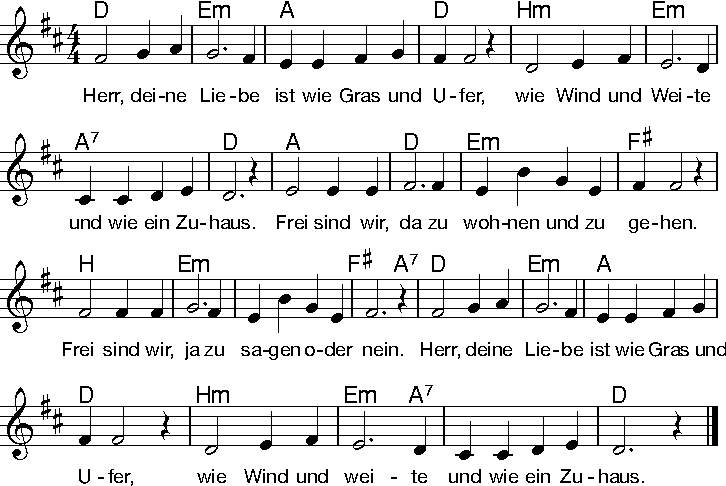
\includegraphics[draft=false, width=1\textwidth]{Noten/Lied111a.pdf}

\beginverse\memorize
\[D]Wir wollen \[Em]Freiheit, \[A]um uns selbst zu \[D]finden,
\[Hm]Freiheit, aus \[Em]der man \[A7]etwas machen \[D]kann.
\[A]Freiheit, die \[D]auch noch \[Em]offen ist für \[F#]Träume,
\[H]wo Baum und \[Em]Blume \[F#]Wurzeln schlagen \[A7]kann.
\endverse

\beginchorus
\[D]Herr, deine \[Em]Liebe \[A]ist wie Gras und \[D]Ufer,
\[Hm]wie Wind und \[Em]Weite \[A7]und wie ein Zu\[D]haus.
\endchorus

\beginverse
^Und dennoch ^sind da ^Mauern zwischen ^Menschen
^und nur durch ^Gitter ^sehen wir uns ^an.
^Unser ver^sklavtes ^Ich ist ein Ge^fängnis
^und ist ge^baut aus ^Steinen uns'rer ^Angst.
\endverse

\printchorus

\beginverse
^Herr, du bist ^Richter, ^Du nur kannst be^freien.
^Wenn du uns ^freisprichst, ^dann ist Freiheit ^da.
^Freiheit, sie ^gilt für ^Menschen, Völker, ^Rassen,
^soweit wie ^deine ^Liebe uns er^greift.
\endverse

\printchorus

\endsong

\beginscripture{}
Ernst Hansen schreibt den Titel im Jahre 1970 nach dem schwedischen "{}Guds kärlek är som stranden och som gräset"{} von Anders Frostenson (1968).
\endscripture
